\section{Kuantifier Universal dan Eksistensial}

Kuantifier adalah operator yang mengikat variabel dan menyatakan seberapa banyak objek dalam domain yang memenuhi predikat tertentu \cite{rosen2019,forallx}. \textbf{Kuantifier universal} $\forall x \, P(x)$ dibaca ``untuk semua $x$, $P(x)$ benar'' atau ``untuk setiap $x$, $P(x)$ berlaku''. \textbf{Kuantifier eksistensial} $\exists x \, P(x)$ dibaca ``terdapat $x$ sehingga $P(x)$ benar'' atau ``ada (sedikitnya satu) $x$ yang memenuhi $P(x)$'' \cite{copi2014,iep_predicate}. Perbedaan fundamental antara keduanya: $\forall$ menuntut bahwa predikat benar untuk \emph{semua} elemen domain, sedangkan $\exists$ hanya membutuhkan \emph{minimal satu} elemen yang memenuhi predikat \cite{wiki_fol,berkeley_fol}.

Semantik kuantifier bergantung pada domain yang dipilih \cite{rosen2019,forallx}. Tabel~\ref{tab:semantik-kuantifier} merangkum kondisi kebenaran untuk $\forall x \, P(x)$ dan $\exists x \, P(x)$.

\begin{table}[htbp]
\centering
\small
\begin{tabular}{|>{\raggedright\arraybackslash}p{2.4cm}|>{\raggedright\arraybackslash}p{3.2cm}|>{\raggedright\arraybackslash}p{3.6cm}|>{\raggedright\arraybackslash}p{2.2cm}|}
\hline
\textbf{Kuantifier} & \textbf{Bacaan} & \textbf{Benar iff} & \textbf{Domain kosong} \\
\hline
$\forall x \, P(x)$ & Untuk semua $x$, $P(x)$ & $P(a)$ benar untuk \emph{semua} $a$ & Benar (vacuously) \\
\hline
$\exists x \, P(x)$ & Ada $x$ sehingga $P(x)$ & Ada \emph{minimal satu} $a$ dengan $P(a)$ benar & Salah \\
\hline
\end{tabular}
\caption{Semantik kuantifier universal dan eksistensial \cite{rosen2019,olp_fol}}
\label{tab:semantik-kuantifier}
\end{table}

Pernyataan $\forall x \, P(x)$ bernilai benar jika dan hanya jika $P(a)$ benar untuk setiap elemen $a$ dalam domain. Pernyataan $\exists x \, P(x)$ bernilai benar jika dan hanya jika terdapat minimal satu elemen $a$ dalam domain sedemikian sehingga $P(a)$ benar \cite{olp_fol,setslogic}. Untuk domain kosong, secara konvensi $\forall x \, P(x)$ dianggap benar (vacuously true) dan $\exists x \, P(x)$ dianggap salah. Dalam praktik, domain biasanya diasumsikan tak kosong \cite{rosen2019}.

Gambar~\ref{fig:forall-vs-exists} mengilustrasikan interpretasi $\forall$ (seluruh domain memenuhi $P$) versus $\exists$ (minimal satu elemen memenuhi $P$) pada domain berhingga \cite{berkeley_fol,brilliant_quantifiers}.

\begin{figure}[htbp]
\centering
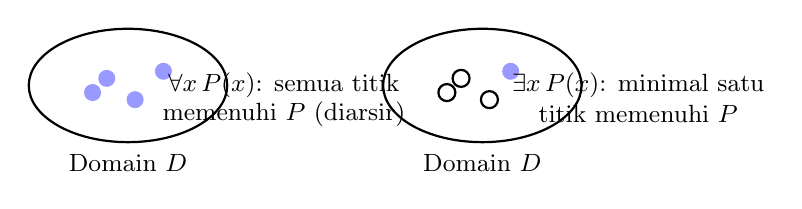
\begin{tikzpicture}[scale=0.9, font=\small]
  % Domain: 4 points
  \draw[thick] (0,0) ellipse (1.4 and 0.8);
  \node at (0,-1.1) {Domain $D$};
  \foreach \x/\y in {0.5/0.2, -0.3/0.1, 0.1/-0.2, -0.5/-0.1} {
    \fill[blue!40] (\x,\y) circle (0.12);
  }
  \node at (2.2,0) {$\forall x \, P(x)$: semua titik};
  \node at (2.2,-0.4) {memenuhi $P$ (diarsir)};

  \begin{scope}[xshift=5cm]
  \draw[thick] (0,0) ellipse (1.4 and 0.8);
  \node at (0,-1.1) {Domain $D$};
  \fill[blue!40] (0.4,0.2) circle (0.12);
  \draw[thick,fill=white] (-0.3,0.1) circle (0.12);
  \draw[thick,fill=white] (0.1,-0.2) circle (0.12);
  \draw[thick,fill=white] (-0.5,-0.1) circle (0.12);
  \node at (2.2,0) {$\exists x \, P(x)$: minimal satu};
  \node at (2.2,-0.4) {titik memenuhi $P$};
  \end{scope}
\end{tikzpicture}
\caption{Interpretasi $\forall x \, P(x)$ (kiri: semua elemen memenuhi $P$) vs $\exists x \, P(x)$ (kanan: minimal satu elemen memenuhi $P$)}
\label{fig:forall-vs-exists}
\end{figure}

Mengevaluasi kebenaran pernyataan berkuantifier membutuhkan pemeriksaan sistematis \cite{levin_discrete,rosen2019}. Untuk $\forall x \, P(x)$: periksa setiap elemen domain; jika ada satu saja yang membuat $P(x)$ salah, maka pernyataan salah. Untuk $\exists x \, P(x)$: cukup temukan satu elemen yang membuat $P(x)$ benar; jika tidak ada satupun, pernyataan salah. Untuk domain finite, evaluasi dapat dilakukan secara eksplisit; untuk domain infinite seperti bilangan asli, kita sering membutuhkan pembuktian \cite{stanford_intrologic,iep_predicate}.

Kuantifier terbatas (bounded quantifiers) muncul ketika kita membatasi perhatian pada subhimpunan domain \cite{forallx,rosen2019}. Tabel~\ref{tab:pola-terjemahan} merangkum pola terjemahan standar untuk ``semua A adalah B'' dan ``ada A yang B'' \cite{stanford_intrologic,berkeley_fol}.

\begin{table}[htbp]
\centering
\small
\begin{tabular}{|>{\raggedright\arraybackslash}p{3.2cm}|l|>{\raggedright\arraybackslash}p{4cm}|}
\hline
\textbf{Pernyataan bahasa alami} & \textbf{Formal} & \textbf{Contoh singkat} \\
\hline
Semua $A$ adalah $B$ & $\forall x \, (A(x) \rightarrow B(x))$ & Semua mahasiswa lulus $\rightarrow$ $\forall x \, (M(x) \to L(x))$ \\
\hline
Ada $A$ yang $B$ & $\exists x \, (A(x) \wedge B(x))$ & Ada bilangan prima genap $\rightarrow$ $\exists x \, (P(x) \wedge G(x))$ \\
\hline
\end{tabular}
\caption{Pola terjemahan kuantifier terbatas \cite{forallx,copi2014}}
\label{tab:pola-terjemahan}
\end{table}

Pernyataan ``Semua mahasiswa rajin belajar'' tidak berarti $\forall x \, P(x)$ jika $P(x)$ = ``$x$ rajin belajar'' dan domain adalah semua manusia; yang benar adalah membatasi $x$ pada mahasiswa. Kesalahan umum: menulis $\forall x \, (Q(x) \wedge P(x))$ untuk ``semua Q adalah P''; bentuk ini salah karena menuntut bahwa setiap $x$ (dalam seluruh domain) memenuhi $Q$ dan $P$, bukan hanya yang memenuhi $Q$ \cite{forallx,copi2014}.

\begin{itemize}
  \item \textbf{Kuantifier Universal} $\forall x \, P(x)$: ``Untuk semua $x$, $P(x)$ benar.'' Benar iff $P(a)$ benar untuk setiap $a$ dalam domain.
  \item \textbf{Kuantifier Eksistensial} $\exists x \, P(x)$: ``Terdapat $x$ sehingga $P(x)$ benar.'' Benar iff ada minimal satu $a$ dalam domain dengan $P(a)$ benar.
\end{itemize}

\begin{contoh}
Misal domain = bilangan bulat positif. Maka $\forall x \, (x > 0)$ benar karena setiap bilangan bulat positif memang lebih besar dari nol. Pernyataan $\exists x \, (x^2 = 4)$ benar karena $x = 2$ memenuhi $x^2 = 4$. Namun $\forall x \, (x^2 = 4)$ salah karena misalnya $x = 3$ tidak memenuhi, dan $\exists x \, (x^2 = -1)$ salah jika domain bilangan real (tidak ada bilangan real yang kuadratnya negatif).
\end{contoh}

\begin{contoh}
\textbf{Evaluasi $\forall$ dan $\exists$ dengan Python} \cite{python_docs_boolean,rosen2019}

Fungsi berikut menerima domain (list) dan predikat (fungsi), lalu mengevaluasi ``untuk semua $x$, $P(x)$'' dan ``ada $x$ sehingga $P(x)$''. Ini langsung merealisasikan semantik kuantifier pada domain berhingga.

\begin{lstlisting}[style=pythonstyle, caption={Evaluasi kuantifier universal dan eksistensial pada domain diskret}]
def forall(domain, predicate):
    """True iff P(a) untuk setiap a dalam domain."""
    return all(predicate(x) for x in domain)

def exists(domain, predicate):
    """True iff ada minimal satu a dengan P(a) benar."""
    return any(predicate(x) for x in domain)

domain = [1, 2, 3, 4]
P = lambda x: x > 2   # P(x): x > 2

print("x   P(x)")
for x in domain:
    print(f"{x}   {P(x)}")
# forall(domain, P) -> False (karena P(1)=P(2)=False)
# exists(domain, P)  -> True  (karena P(3)=P(4)=True)
print("forall x P(x):", forall(domain, P))   # False
print("exists x P(x):", exists(domain, P))   # True
\end{lstlisting}
\end{contoh}
